\documentclass[twoside]{book}

% Packages required by doxygen
\usepackage{fixltx2e}
\usepackage{calc}
\usepackage{doxygen}
\usepackage[export]{adjustbox} % also loads graphicx
\usepackage{graphicx}
\usepackage[utf8]{inputenc}
\usepackage{makeidx}
\usepackage{multicol}
\usepackage{multirow}
\PassOptionsToPackage{warn}{textcomp}
\usepackage{textcomp}
\usepackage[nointegrals]{wasysym}
\usepackage[table]{xcolor}

% Font selection
\usepackage[T1]{fontenc}
\usepackage[scaled=.90]{helvet}
\usepackage{courier}
\usepackage{amssymb}
\usepackage{sectsty}
\renewcommand{\familydefault}{\sfdefault}
\allsectionsfont{%
  \fontseries{bc}\selectfont%
  \color{darkgray}%
}
\renewcommand{\DoxyLabelFont}{%
  \fontseries{bc}\selectfont%
  \color{darkgray}%
}
\newcommand{\+}{\discretionary{\mbox{\scriptsize$\hookleftarrow$}}{}{}}

% Page & text layout
\usepackage{geometry}
\geometry{%
  a4paper,%
  top=2.5cm,%
  bottom=2.5cm,%
  left=2.5cm,%
  right=2.5cm%
}
\tolerance=750
\hfuzz=15pt
\hbadness=750
\setlength{\emergencystretch}{15pt}
\setlength{\parindent}{0cm}
\setlength{\parskip}{3ex plus 2ex minus 2ex}
\makeatletter
\renewcommand{\paragraph}{%
  \@startsection{paragraph}{4}{0ex}{-1.0ex}{1.0ex}{%
    \normalfont\normalsize\bfseries\SS@parafont%
  }%
}
\renewcommand{\subparagraph}{%
  \@startsection{subparagraph}{5}{0ex}{-1.0ex}{1.0ex}{%
    \normalfont\normalsize\bfseries\SS@subparafont%
  }%
}
\makeatother

% Headers & footers
\usepackage{fancyhdr}
\pagestyle{fancyplain}
\fancyhead[LE]{\fancyplain{}{\bfseries\thepage}}
\fancyhead[CE]{\fancyplain{}{}}
\fancyhead[RE]{\fancyplain{}{\bfseries\leftmark}}
\fancyhead[LO]{\fancyplain{}{\bfseries\rightmark}}
\fancyhead[CO]{\fancyplain{}{}}
\fancyhead[RO]{\fancyplain{}{\bfseries\thepage}}
\fancyfoot[LE]{\fancyplain{}{}}
\fancyfoot[CE]{\fancyplain{}{}}
\fancyfoot[RE]{\fancyplain{}{\bfseries\scriptsize Generated by Doxygen }}
\fancyfoot[LO]{\fancyplain{}{\bfseries\scriptsize Generated by Doxygen }}
\fancyfoot[CO]{\fancyplain{}{}}
\fancyfoot[RO]{\fancyplain{}{}}
\renewcommand{\footrulewidth}{0.4pt}
\renewcommand{\chaptermark}[1]{%
  \markboth{#1}{}%
}
\renewcommand{\sectionmark}[1]{%
  \markright{\thesection\ #1}%
}

% Indices & bibliography
\usepackage{natbib}
\usepackage[titles]{tocloft}
\setcounter{tocdepth}{3}
\setcounter{secnumdepth}{5}
\makeindex

% Hyperlinks (required, but should be loaded last)
\usepackage{ifpdf}
\ifpdf
  \usepackage[pdftex,pagebackref=true]{hyperref}
\else
  \usepackage[ps2pdf,pagebackref=true]{hyperref}
\fi
\hypersetup{%
  colorlinks=true,%
  linkcolor=blue,%
  citecolor=blue,%
  unicode%
}

% Custom commands
\newcommand{\clearemptydoublepage}{%
  \newpage{\pagestyle{empty}\cleardoublepage}%
}

\usepackage{caption}
\captionsetup{labelsep=space,justification=centering,font={bf},singlelinecheck=off,skip=4pt,position=top}

%===== C O N T E N T S =====

\begin{document}

% Titlepage & ToC
\hypersetup{pageanchor=false,
             bookmarksnumbered=true,
             pdfencoding=unicode
            }
\pagenumbering{alph}
\begin{titlepage}
\vspace*{7cm}
\begin{center}%
{\Large My Project }\\
\vspace*{1cm}
{\large Generated by Doxygen 1.8.13}\\
\end{center}
\end{titlepage}
\clearemptydoublepage
\pagenumbering{roman}
\tableofcontents
\clearemptydoublepage
\pagenumbering{arabic}
\hypersetup{pageanchor=true}

%--- Begin generated contents ---
\chapter{C\+S-\/3560-\/final-\/part2}
\label{md_README}
\Hypertarget{md_README}
\input{md_README}
\chapter{Hierarchical Index}
\section{Class Hierarchy}
This inheritance list is sorted roughly, but not completely, alphabetically\+:\begin{DoxyCompactList}
\item exception\begin{DoxyCompactList}
\item \contentsline{section}{Catch\+:\+:Benchmark\+:\+:Detail\+:\+:optimized\+\_\+away\+\_\+error}{\pageref{structCatch_1_1Benchmark_1_1Detail_1_1optimized__away__error}}{}
\end{DoxyCompactList}
\item I\+Generator\+Tracker\begin{DoxyCompactList}
\item \contentsline{section}{Catch\+:\+:Generators\+:\+:Generator\+Tracker}{\pageref{structCatch_1_1Generators_1_1GeneratorTracker}}{}
\end{DoxyCompactList}
\item I\+Mutable\+Context\begin{DoxyCompactList}
\item \contentsline{section}{Catch\+:\+:Context}{\pageref{classCatch_1_1Context}}{}
\end{DoxyCompactList}
\item Non\+Copyable\begin{DoxyCompactList}
\item \contentsline{section}{Catch\+:\+:Context}{\pageref{classCatch_1_1Context}}{}
\end{DoxyCompactList}
\item \contentsline{section}{Catch\+:\+:String\+Streams}{\pageref{structCatch_1_1StringStreams}}{}
\item \contentsline{section}{Catch\+:\+:Summary\+Column}{\pageref{structCatch_1_1SummaryColumn}}{}
\item \contentsline{section}{Catch\+:\+:Table\+Printer}{\pageref{classCatch_1_1TablePrinter}}{}
\item Tracker\+Base\begin{DoxyCompactList}
\item \contentsline{section}{Catch\+:\+:Generators\+:\+:Generator\+Tracker}{\pageref{structCatch_1_1Generators_1_1GeneratorTracker}}{}
\end{DoxyCompactList}
\end{DoxyCompactList}

\chapter{Class Index}
\section{Class List}
Here are the classes, structs, unions and interfaces with brief descriptions\+:\begin{DoxyCompactList}
\item\contentsline{section}{\hyperlink{classCatch_1_1Context}{Catch\+::\+Context} }{\pageref{classCatch_1_1Context}}{}
\item\contentsline{section}{\hyperlink{structCatch_1_1Generators_1_1GeneratorTracker}{Catch\+::\+Generators\+::\+Generator\+Tracker} }{\pageref{structCatch_1_1Generators_1_1GeneratorTracker}}{}
\item\contentsline{section}{\hyperlink{structCatch_1_1Benchmark_1_1Detail_1_1optimized__away__error}{Catch\+::\+Benchmark\+::\+Detail\+::optimized\+\_\+away\+\_\+error} }{\pageref{structCatch_1_1Benchmark_1_1Detail_1_1optimized__away__error}}{}
\item\contentsline{section}{\hyperlink{structCatch_1_1StringStreams}{Catch\+::\+String\+Streams} }{\pageref{structCatch_1_1StringStreams}}{}
\item\contentsline{section}{\hyperlink{structCatch_1_1SummaryColumn}{Catch\+::\+Summary\+Column} }{\pageref{structCatch_1_1SummaryColumn}}{}
\item\contentsline{section}{\hyperlink{classCatch_1_1TablePrinter}{Catch\+::\+Table\+Printer} }{\pageref{classCatch_1_1TablePrinter}}{}
\end{DoxyCompactList}

\chapter{File Index}
\section{File List}
Here is a list of all documented files with brief descriptions\+:\begin{DoxyCompactList}
\item\contentsline{section}{\hyperlink{catch__amalgamated_8cc}{catch\+\_\+amalgamated.\+cc} }{\pageref{catch__amalgamated_8cc}}{}
\item\contentsline{section}{\hyperlink{function_8h}{function.\+h} \\*Library containing count\+Lines and count\+Char }{\pageref{function_8h}}{}
\item\contentsline{section}{\hyperlink{main_8cc}{main.\+cc} \\*Main file }{\pageref{main_8cc}}{}
\end{DoxyCompactList}

\chapter{Class Documentation}
\hypertarget{classCatch_1_1Context}{}\section{Catch\+:\+:Context Class Reference}
\label{classCatch_1_1Context}\index{Catch\+::\+Context@{Catch\+::\+Context}}


Inheritance diagram for Catch\+:\+:Context\+:
\nopagebreak
\begin{figure}[H]
\begin{center}
\leavevmode
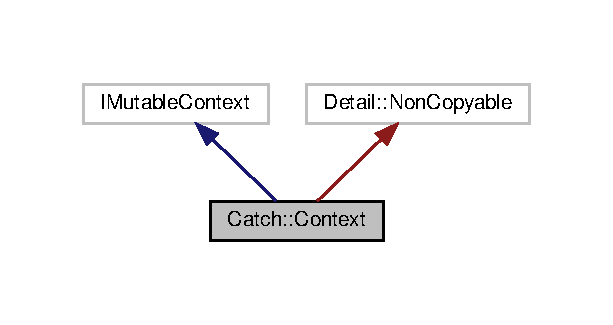
\includegraphics[width=294pt]{classCatch_1_1Context__inherit__graph}
\end{center}
\end{figure}


Collaboration diagram for Catch\+:\+:Context\+:
\nopagebreak
\begin{figure}[H]
\begin{center}
\leavevmode
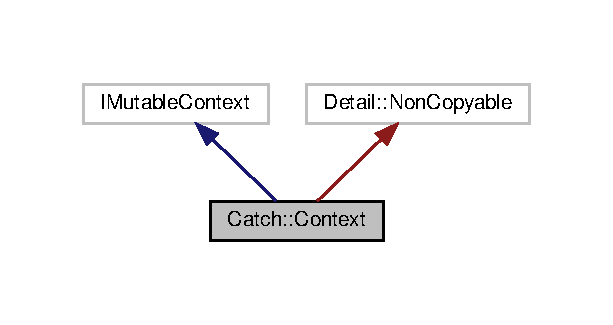
\includegraphics[width=294pt]{classCatch_1_1Context__coll__graph}
\end{center}
\end{figure}
\subsection*{Public Member Functions}
\begin{DoxyCompactItemize}
\item 
\mbox{\Hypertarget{classCatch_1_1Context_aead6db73ac48bfc8043946de905de2fc}\label{classCatch_1_1Context_aead6db73ac48bfc8043946de905de2fc}} 
I\+Result\+Capture $\ast$ {\bfseries get\+Result\+Capture} () override
\item 
\mbox{\Hypertarget{classCatch_1_1Context_a308cedbf37adc981d78ea8c3fd4d2793}\label{classCatch_1_1Context_a308cedbf37adc981d78ea8c3fd4d2793}} 
I\+Runner $\ast$ {\bfseries get\+Runner} () override
\item 
\mbox{\Hypertarget{classCatch_1_1Context_a9a7650605bcb44da52769c4760a83a74}\label{classCatch_1_1Context_a9a7650605bcb44da52769c4760a83a74}} 
I\+Config const  $\ast$ {\bfseries get\+Config} () const override
\item 
\mbox{\Hypertarget{classCatch_1_1Context_a3845fb318b9d6ee96961d9013ee8c0ef}\label{classCatch_1_1Context_a3845fb318b9d6ee96961d9013ee8c0ef}} 
void {\bfseries set\+Result\+Capture} (I\+Result\+Capture $\ast$result\+Capture) override
\item 
\mbox{\Hypertarget{classCatch_1_1Context_ab689f97687dd626f89e8a208c4903f97}\label{classCatch_1_1Context_ab689f97687dd626f89e8a208c4903f97}} 
void {\bfseries set\+Runner} (I\+Runner $\ast$runner) override
\item 
\mbox{\Hypertarget{classCatch_1_1Context_a0fcec7be2d1f1a7591b6ee559d03afc9}\label{classCatch_1_1Context_a0fcec7be2d1f1a7591b6ee559d03afc9}} 
void {\bfseries set\+Config} (I\+Config const $\ast$config) override
\end{DoxyCompactItemize}
\subsection*{Friends}
\begin{DoxyCompactItemize}
\item 
\mbox{\Hypertarget{classCatch_1_1Context_aea4b25692aaf4397cdf630716976f6b8}\label{classCatch_1_1Context_aea4b25692aaf4397cdf630716976f6b8}} 
I\+Mutable\+Context \& {\bfseries get\+Current\+Mutable\+Context} ()
\end{DoxyCompactItemize}


The documentation for this class was generated from the following file\+:\begin{DoxyCompactItemize}
\item 
\hyperlink{catch__amalgamated_8cc}{catch\+\_\+amalgamated.\+cc}\end{DoxyCompactItemize}

\hypertarget{structCatch_1_1Generators_1_1GeneratorTracker}{}\section{Catch\+:\+:Generators\+:\+:Generator\+Tracker Struct Reference}
\label{structCatch_1_1Generators_1_1GeneratorTracker}\index{Catch\+::\+Generators\+::\+Generator\+Tracker@{Catch\+::\+Generators\+::\+Generator\+Tracker}}


Inheritance diagram for Catch\+:\+:Generators\+:\+:Generator\+Tracker\+:
\nopagebreak
\begin{figure}[H]
\begin{center}
\leavevmode
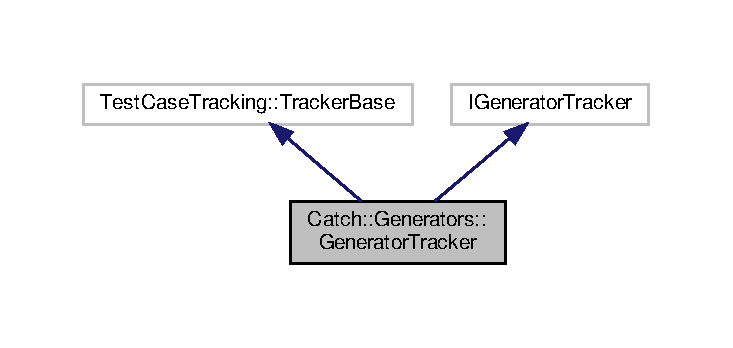
\includegraphics[width=350pt]{structCatch_1_1Generators_1_1GeneratorTracker__inherit__graph}
\end{center}
\end{figure}


Collaboration diagram for Catch\+:\+:Generators\+:\+:Generator\+Tracker\+:
\nopagebreak
\begin{figure}[H]
\begin{center}
\leavevmode
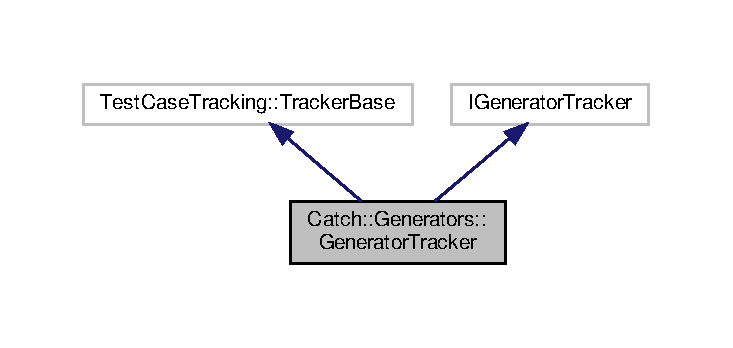
\includegraphics[width=350pt]{structCatch_1_1Generators_1_1GeneratorTracker__coll__graph}
\end{center}
\end{figure}
\subsection*{Public Member Functions}
\begin{DoxyCompactItemize}
\item 
\mbox{\Hypertarget{structCatch_1_1Generators_1_1GeneratorTracker_aa70d62ac075d47401cfad669fbb15057}\label{structCatch_1_1Generators_1_1GeneratorTracker_aa70d62ac075d47401cfad669fbb15057}} 
{\bfseries Generator\+Tracker} (Test\+Case\+Tracking\+::\+Name\+And\+Location const \&name\+And\+Location, Tracker\+Context \&ctx, I\+Tracker $\ast$parent)
\item 
\mbox{\Hypertarget{structCatch_1_1Generators_1_1GeneratorTracker_a58f3a500872cec6bfd1c9e605c06294f}\label{structCatch_1_1Generators_1_1GeneratorTracker_a58f3a500872cec6bfd1c9e605c06294f}} 
bool {\bfseries is\+Generator\+Tracker} () const override
\item 
\mbox{\Hypertarget{structCatch_1_1Generators_1_1GeneratorTracker_ae798faa657dc7eba5b1e866cfe824a4b}\label{structCatch_1_1Generators_1_1GeneratorTracker_ae798faa657dc7eba5b1e866cfe824a4b}} 
auto {\bfseries has\+Generator} () const -\/$>$ bool override
\item 
\mbox{\Hypertarget{structCatch_1_1Generators_1_1GeneratorTracker_afb933cbb4007f63adb137bd961836165}\label{structCatch_1_1Generators_1_1GeneratorTracker_afb933cbb4007f63adb137bd961836165}} 
void {\bfseries close} () override
\item 
\mbox{\Hypertarget{structCatch_1_1Generators_1_1GeneratorTracker_a902884030ef21d5eca2e7b78e36750c5}\label{structCatch_1_1Generators_1_1GeneratorTracker_a902884030ef21d5eca2e7b78e36750c5}} 
auto {\bfseries get\+Generator} () const -\/$>$ Generator\+Base\+Ptr const \&override
\item 
\mbox{\Hypertarget{structCatch_1_1Generators_1_1GeneratorTracker_a89ebb06a194997b2870e258b609ea296}\label{structCatch_1_1Generators_1_1GeneratorTracker_a89ebb06a194997b2870e258b609ea296}} 
void {\bfseries set\+Generator} (Generator\+Base\+Ptr \&\&generator) override
\end{DoxyCompactItemize}
\subsection*{Static Public Member Functions}
\begin{DoxyCompactItemize}
\item 
\mbox{\Hypertarget{structCatch_1_1Generators_1_1GeneratorTracker_a57ee9aa54af9ca7d9d97b14affcf0d99}\label{structCatch_1_1Generators_1_1GeneratorTracker_a57ee9aa54af9ca7d9d97b14affcf0d99}} 
static \hyperlink{structCatch_1_1Generators_1_1GeneratorTracker}{Generator\+Tracker} \& {\bfseries acquire} (Tracker\+Context \&ctx, Test\+Case\+Tracking\+::\+Name\+And\+Location const \&name\+And\+Location)
\end{DoxyCompactItemize}
\subsection*{Public Attributes}
\begin{DoxyCompactItemize}
\item 
\mbox{\Hypertarget{structCatch_1_1Generators_1_1GeneratorTracker_a498ea8e6ace9976202f69600f00a3df2}\label{structCatch_1_1Generators_1_1GeneratorTracker_a498ea8e6ace9976202f69600f00a3df2}} 
Generator\+Base\+Ptr {\bfseries m\+\_\+generator}
\end{DoxyCompactItemize}


The documentation for this struct was generated from the following file\+:\begin{DoxyCompactItemize}
\item 
\hyperlink{catch__amalgamated_8cc}{catch\+\_\+amalgamated.\+cc}\end{DoxyCompactItemize}

\hypertarget{structCatch_1_1Benchmark_1_1Detail_1_1optimized__away__error}{}\section{Catch\+:\+:Benchmark\+:\+:Detail\+:\+:optimized\+\_\+away\+\_\+error Struct Reference}
\label{structCatch_1_1Benchmark_1_1Detail_1_1optimized__away__error}\index{Catch\+::\+Benchmark\+::\+Detail\+::optimized\+\_\+away\+\_\+error@{Catch\+::\+Benchmark\+::\+Detail\+::optimized\+\_\+away\+\_\+error}}


Inheritance diagram for Catch\+:\+:Benchmark\+:\+:Detail\+:\+:optimized\+\_\+away\+\_\+error\+:
\nopagebreak
\begin{figure}[H]
\begin{center}
\leavevmode
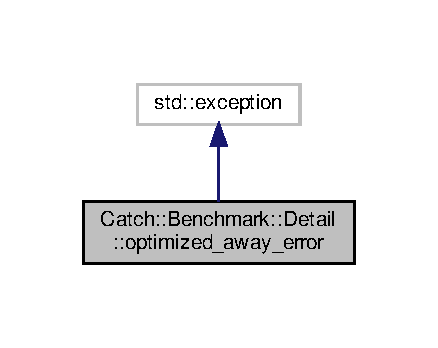
\includegraphics[width=210pt]{structCatch_1_1Benchmark_1_1Detail_1_1optimized__away__error__inherit__graph}
\end{center}
\end{figure}


Collaboration diagram for Catch\+:\+:Benchmark\+:\+:Detail\+:\+:optimized\+\_\+away\+\_\+error\+:
\nopagebreak
\begin{figure}[H]
\begin{center}
\leavevmode
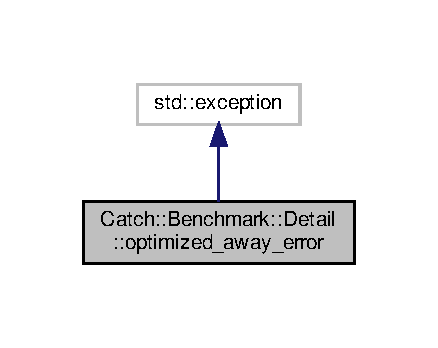
\includegraphics[width=210pt]{structCatch_1_1Benchmark_1_1Detail_1_1optimized__away__error__coll__graph}
\end{center}
\end{figure}
\subsection*{Public Member Functions}
\begin{DoxyCompactItemize}
\item 
\mbox{\Hypertarget{structCatch_1_1Benchmark_1_1Detail_1_1optimized__away__error_a77667d73ffbd8b79a29c638000cf7990}\label{structCatch_1_1Benchmark_1_1Detail_1_1optimized__away__error_a77667d73ffbd8b79a29c638000cf7990}} 
const char $\ast$ {\bfseries what} () const noexcept override
\end{DoxyCompactItemize}


The documentation for this struct was generated from the following file\+:\begin{DoxyCompactItemize}
\item 
\hyperlink{catch__amalgamated_8cc}{catch\+\_\+amalgamated.\+cc}\end{DoxyCompactItemize}

\hypertarget{structCatch_1_1StringStreams}{}\section{Catch\+:\+:String\+Streams Struct Reference}
\label{structCatch_1_1StringStreams}\index{Catch\+::\+String\+Streams@{Catch\+::\+String\+Streams}}
\subsection*{Public Member Functions}
\begin{DoxyCompactItemize}
\item 
\mbox{\Hypertarget{structCatch_1_1StringStreams_a1e98cd696f9e141b3a89f305af962d91}\label{structCatch_1_1StringStreams_a1e98cd696f9e141b3a89f305af962d91}} 
auto {\bfseries add} () -\/$>$ std\+::size\+\_\+t
\item 
\mbox{\Hypertarget{structCatch_1_1StringStreams_a7e746fe736750cd67389883f6787a9b7}\label{structCatch_1_1StringStreams_a7e746fe736750cd67389883f6787a9b7}} 
void {\bfseries release} (std\+::size\+\_\+t index)
\end{DoxyCompactItemize}
\subsection*{Public Attributes}
\begin{DoxyCompactItemize}
\item 
\mbox{\Hypertarget{structCatch_1_1StringStreams_a12e806f1886bc1d2ea8e29c13a9b38ca}\label{structCatch_1_1StringStreams_a12e806f1886bc1d2ea8e29c13a9b38ca}} 
std\+::vector$<$ Detail\+::unique\+\_\+ptr$<$ std\+::ostringstream $>$ $>$ {\bfseries m\+\_\+streams}
\item 
\mbox{\Hypertarget{structCatch_1_1StringStreams_a6c04fb72aa5c9eb66af33a56857f996f}\label{structCatch_1_1StringStreams_a6c04fb72aa5c9eb66af33a56857f996f}} 
std\+::vector$<$ std\+::size\+\_\+t $>$ {\bfseries m\+\_\+unused}
\item 
\mbox{\Hypertarget{structCatch_1_1StringStreams_a3eee987f15e8bd678b751cf0a1702a03}\label{structCatch_1_1StringStreams_a3eee987f15e8bd678b751cf0a1702a03}} 
std\+::ostringstream {\bfseries m\+\_\+reference\+Stream}
\end{DoxyCompactItemize}


The documentation for this struct was generated from the following file\+:\begin{DoxyCompactItemize}
\item 
\hyperlink{catch__amalgamated_8cc}{catch\+\_\+amalgamated.\+cc}\end{DoxyCompactItemize}

\hypertarget{structCatch_1_1SummaryColumn}{}\section{Catch\+:\+:Summary\+Column Struct Reference}
\label{structCatch_1_1SummaryColumn}\index{Catch\+::\+Summary\+Column@{Catch\+::\+Summary\+Column}}
\subsection*{Public Member Functions}
\begin{DoxyCompactItemize}
\item 
\mbox{\Hypertarget{structCatch_1_1SummaryColumn_a5ccb6d3a534033e95fe8624494a5330b}\label{structCatch_1_1SummaryColumn_a5ccb6d3a534033e95fe8624494a5330b}} 
{\bfseries Summary\+Column} (std\+::string \+\_\+label, Colour\+::\+Code \+\_\+colour)
\item 
\mbox{\Hypertarget{structCatch_1_1SummaryColumn_aed5c921b3ad08f653d879280be435d1a}\label{structCatch_1_1SummaryColumn_aed5c921b3ad08f653d879280be435d1a}} 
\hyperlink{structCatch_1_1SummaryColumn}{Summary\+Column} {\bfseries add\+Row} (std\+::size\+\_\+t count)
\end{DoxyCompactItemize}
\subsection*{Public Attributes}
\begin{DoxyCompactItemize}
\item 
\mbox{\Hypertarget{structCatch_1_1SummaryColumn_a01f1eaae714a8f53494ad6e0926a1157}\label{structCatch_1_1SummaryColumn_a01f1eaae714a8f53494ad6e0926a1157}} 
std\+::string {\bfseries label}
\item 
\mbox{\Hypertarget{structCatch_1_1SummaryColumn_adeb1eac3b0eda3b653c9063a2fe521d7}\label{structCatch_1_1SummaryColumn_adeb1eac3b0eda3b653c9063a2fe521d7}} 
Colour\+::\+Code {\bfseries colour}
\item 
\mbox{\Hypertarget{structCatch_1_1SummaryColumn_ad0f54e7422f5773b03e96d0019915f8d}\label{structCatch_1_1SummaryColumn_ad0f54e7422f5773b03e96d0019915f8d}} 
std\+::vector$<$ std\+::string $>$ {\bfseries rows}
\end{DoxyCompactItemize}


The documentation for this struct was generated from the following file\+:\begin{DoxyCompactItemize}
\item 
\hyperlink{catch__amalgamated_8cc}{catch\+\_\+amalgamated.\+cc}\end{DoxyCompactItemize}

\hypertarget{classCatch_1_1TablePrinter}{}\section{Catch\+:\+:Table\+Printer Class Reference}
\label{classCatch_1_1TablePrinter}\index{Catch\+::\+Table\+Printer@{Catch\+::\+Table\+Printer}}
\subsection*{Public Member Functions}
\begin{DoxyCompactItemize}
\item 
\mbox{\Hypertarget{classCatch_1_1TablePrinter_a5927152ae95eeefa471ab27c01644980}\label{classCatch_1_1TablePrinter_a5927152ae95eeefa471ab27c01644980}} 
{\bfseries Table\+Printer} (std\+::ostream \&os, std\+::vector$<$ Column\+Info $>$ column\+Infos)
\item 
\mbox{\Hypertarget{classCatch_1_1TablePrinter_a378f2bdf7f353a13d3a9f683a2c1fa04}\label{classCatch_1_1TablePrinter_a378f2bdf7f353a13d3a9f683a2c1fa04}} 
auto {\bfseries column\+Infos} () const -\/$>$ std\+::vector$<$ Column\+Info $>$ const \&
\item 
\mbox{\Hypertarget{classCatch_1_1TablePrinter_abb4f12add189af81ef29694014cac6df}\label{classCatch_1_1TablePrinter_abb4f12add189af81ef29694014cac6df}} 
void {\bfseries open} ()
\item 
\mbox{\Hypertarget{classCatch_1_1TablePrinter_aa5936978a607e853ac0346df60e0f6f7}\label{classCatch_1_1TablePrinter_aa5936978a607e853ac0346df60e0f6f7}} 
void {\bfseries close} ()
\end{DoxyCompactItemize}
\subsection*{Friends}
\begin{DoxyCompactItemize}
\item 
\mbox{\Hypertarget{classCatch_1_1TablePrinter_a78f9037858dee3e7c685f189e645289f}\label{classCatch_1_1TablePrinter_a78f9037858dee3e7c685f189e645289f}} 
{\footnotesize template$<$typename T $>$ }\\\hyperlink{classCatch_1_1TablePrinter}{Table\+Printer} \& {\bfseries operator$<$$<$} (\hyperlink{classCatch_1_1TablePrinter}{Table\+Printer} \&tp, T const \&value)
\item 
\mbox{\Hypertarget{classCatch_1_1TablePrinter_aa2ec1ab18690d49a9bf57aea1b0dfdd7}\label{classCatch_1_1TablePrinter_aa2ec1ab18690d49a9bf57aea1b0dfdd7}} 
\hyperlink{classCatch_1_1TablePrinter}{Table\+Printer} \& {\bfseries operator$<$$<$} (\hyperlink{classCatch_1_1TablePrinter}{Table\+Printer} \&tp, Column\+Break)
\item 
\mbox{\Hypertarget{classCatch_1_1TablePrinter_aaab99f8b2c640c880903cc8314925f4d}\label{classCatch_1_1TablePrinter_aaab99f8b2c640c880903cc8314925f4d}} 
\hyperlink{classCatch_1_1TablePrinter}{Table\+Printer} \& {\bfseries operator$<$$<$} (\hyperlink{classCatch_1_1TablePrinter}{Table\+Printer} \&tp, Row\+Break)
\end{DoxyCompactItemize}


The documentation for this class was generated from the following file\+:\begin{DoxyCompactItemize}
\item 
\hyperlink{catch__amalgamated_8cc}{catch\+\_\+amalgamated.\+cc}\end{DoxyCompactItemize}

\chapter{File Documentation}
\hypertarget{catch__amalgamated_8cc}{}\section{catch\+\_\+amalgamated.\+cc File Reference}
\label{catch__amalgamated_8cc}\index{catch\+\_\+amalgamated.\+cc@{catch\+\_\+amalgamated.\+cc}}
{\ttfamily \#include \char`\"{}catch\+\_\+amalgamated.\+hpp\char`\"{}}\newline
{\ttfamily \#include $<$cassert$>$}\newline
{\ttfamily \#include $<$iterator$>$}\newline
{\ttfamily \#include $<$random$>$}\newline
{\ttfamily \#include $<$exception$>$}\newline
{\ttfamily \#include $<$cmath$>$}\newline
{\ttfamily \#include $<$limits$>$}\newline
{\ttfamily \#include $<$stack$>$}\newline
{\ttfamily \#include $<$algorithm$>$}\newline
{\ttfamily \#include $<$iomanip$>$}\newline
{\ttfamily \#include $<$set$>$}\newline
{\ttfamily \#include $<$cctype$>$}\newline
{\ttfamily \#include $<$string$>$}\newline
{\ttfamily \#include $<$vector$>$}\newline
{\ttfamily \#include $<$chrono$>$}\newline
{\ttfamily \#include $<$ostream$>$}\newline
{\ttfamily \#include $<$cerrno$>$}\newline
{\ttfamily \#include $<$fstream$>$}\newline
{\ttfamily \#include $<$ctime$>$}\newline
{\ttfamily \#include $<$cstring$>$}\newline
{\ttfamily \#include $<$unistd.\+h$>$}\newline
{\ttfamily \#include $<$stdexcept$>$}\newline
{\ttfamily \#include $<$cstdio$>$}\newline
{\ttfamily \#include $<$sstream$>$}\newline
{\ttfamily \#include $<$utility$>$}\newline
{\ttfamily \#include $<$iostream$>$}\newline
{\ttfamily \#include $<$cstdint$>$}\newline
{\ttfamily \#include $<$memory$>$}\newline
{\ttfamily \#include $<$type\+\_\+traits$>$}\newline
{\ttfamily \#include $<$cstdlib$>$}\newline
{\ttfamily \#include $<$regex$>$}\newline
{\ttfamily \#include $<$cfloat$>$}\newline
{\ttfamily \#include $<$map$>$}\newline
Include dependency graph for catch\+\_\+amalgamated.\+cc\+:
\nopagebreak
\begin{figure}[H]
\begin{center}
\leavevmode
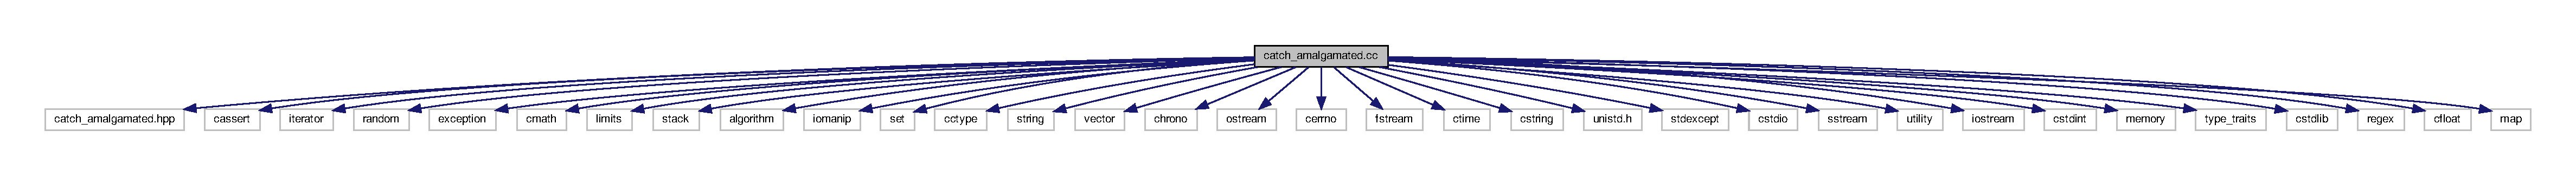
\includegraphics[width=350pt]{catch__amalgamated_8cc__incl}
\end{center}
\end{figure}
\subsection*{Classes}
\begin{DoxyCompactItemize}
\item 
struct \hyperlink{structCatch_1_1Benchmark_1_1Detail_1_1optimized__away__error}{Catch\+::\+Benchmark\+::\+Detail\+::optimized\+\_\+away\+\_\+error}
\item 
class \hyperlink{classCatch_1_1Context}{Catch\+::\+Context}
\item 
struct \hyperlink{structCatch_1_1Generators_1_1GeneratorTracker}{Catch\+::\+Generators\+::\+Generator\+Tracker}
\item 
struct \hyperlink{structCatch_1_1StringStreams}{Catch\+::\+String\+Streams}
\item 
class \hyperlink{classCatch_1_1TablePrinter}{Catch\+::\+Table\+Printer}
\item 
struct \hyperlink{structCatch_1_1SummaryColumn}{Catch\+::\+Summary\+Column}
\end{DoxyCompactItemize}
\subsection*{Typedefs}
\begin{DoxyCompactItemize}
\item 
\mbox{\Hypertarget{catch__amalgamated_8cc_af942e91344c728dbd8c9732dbf8054c9}\label{catch__amalgamated_8cc_af942e91344c728dbd8c9732dbf8054c9}} 
using {\bfseries Catch\+::\+Registry\+Hub\+Singleton} = Singleton$<$ Registry\+Hub, I\+Registry\+Hub, I\+Mutable\+Registry\+Hub $>$
\end{DoxyCompactItemize}
\subsection*{Enumerations}
\begin{DoxyCompactItemize}
\item 
\mbox{\Hypertarget{catch__amalgamated_8cc_a65dcb4c6cc6803847848523398ae680c}\label{catch__amalgamated_8cc_a65dcb4c6cc6803847848523398ae680c}} 
enum {\bfseries Floating\+Point\+Kind} \+: uint8\+\_\+t \{ {\bfseries Float}, 
{\bfseries Double}
 \}
\item 
\mbox{\Hypertarget{catch__amalgamated_8cc_addb676bebb9d4ed3ffeb557e6d083362}\label{catch__amalgamated_8cc_addb676bebb9d4ed3ffeb557e6d083362}} 
enum {\bfseries Justification} \{ {\bfseries Left}, 
{\bfseries Right}
 \}
\end{DoxyCompactItemize}
\subsection*{Functions}
\begin{DoxyCompactItemize}
\item 
\mbox{\Hypertarget{catch__amalgamated_8cc_afc97f2c4454d38848a57445bcc3de5af}\label{catch__amalgamated_8cc_afc97f2c4454d38848a57445bcc3de5af}} 
double {\bfseries Catch\+::\+Benchmark\+::\+Detail\+::weighted\+\_\+average\+\_\+quantile} (int k, int q, std\+::vector$<$ double $>$\+::iterator first, std\+::vector$<$ double $>$\+::iterator last)
\item 
\mbox{\Hypertarget{catch__amalgamated_8cc_a62d6c634e2c8901d02ffe8718817f1b4}\label{catch__amalgamated_8cc_a62d6c634e2c8901d02ffe8718817f1b4}} 
double {\bfseries Catch\+::\+Benchmark\+::\+Detail\+::erfc\+\_\+inv} (double x)
\item 
\mbox{\Hypertarget{catch__amalgamated_8cc_af3527090cdeb0456b1aacbdc29050841}\label{catch__amalgamated_8cc_af3527090cdeb0456b1aacbdc29050841}} 
double {\bfseries Catch\+::\+Benchmark\+::\+Detail\+::normal\+\_\+quantile} (double p)
\item 
\mbox{\Hypertarget{catch__amalgamated_8cc_ab7225b5a34d78c22bc5186297b68aa83}\label{catch__amalgamated_8cc_ab7225b5a34d78c22bc5186297b68aa83}} 
double {\bfseries Catch\+::\+Benchmark\+::\+Detail\+::outlier\+\_\+variance} (Estimate$<$ double $>$ mean, Estimate$<$ double $>$ stddev, int n)
\item 
\mbox{\Hypertarget{catch__amalgamated_8cc_a7ee9e4fb035c7f8fa1cbfd4c3cd6242d}\label{catch__amalgamated_8cc_a7ee9e4fb035c7f8fa1cbfd4c3cd6242d}} 
bootstrap\+\_\+analysis {\bfseries Catch\+::\+Benchmark\+::\+Detail\+::analyse\+\_\+samples} (double confidence\+\_\+level, int n\+\_\+resamples, std\+::vector$<$ double $>$\+::iterator first, std\+::vector$<$ double $>$\+::iterator last)
\item 
\mbox{\Hypertarget{catch__amalgamated_8cc_accb97601fac7308aa9c11dcdb439ddb8}\label{catch__amalgamated_8cc_accb97601fac7308aa9c11dcdb439ddb8}} 
void {\bfseries Catch\+::\+Benchmark\+::\+Detail\+::throw\+\_\+optimized\+\_\+away\+\_\+error} ()
\item 
\mbox{\Hypertarget{catch__amalgamated_8cc_a2c0ddb4f68733f283405e726949456b9}\label{catch__amalgamated_8cc_a2c0ddb4f68733f283405e726949456b9}} 
Approx {\bfseries Catch\+::literals\+::operator\char`\"{}\char`\"{} \+\_\+a} (long double val)
\item 
\mbox{\Hypertarget{catch__amalgamated_8cc_a566b65940e906431543d3349c99098eb}\label{catch__amalgamated_8cc_a566b65940e906431543d3349c99098eb}} 
Approx {\bfseries Catch\+::literals\+::operator\char`\"{}\char`\"{} \+\_\+a} (unsigned long long val)
\item 
\mbox{\Hypertarget{catch__amalgamated_8cc_a6332c92ab0c3952586b22cb96fdb8d44}\label{catch__amalgamated_8cc_a6332c92ab0c3952586b22cb96fdb8d44}} 
I\+Registry\+Hub const  \& {\bfseries Catch\+::get\+Registry\+Hub} ()
\item 
\mbox{\Hypertarget{catch__amalgamated_8cc_ac9ddcc6d66079add9cb2a3140b8ae51e}\label{catch__amalgamated_8cc_ac9ddcc6d66079add9cb2a3140b8ae51e}} 
I\+Mutable\+Registry\+Hub \& {\bfseries Catch\+::get\+Mutable\+Registry\+Hub} ()
\item 
\mbox{\Hypertarget{catch__amalgamated_8cc_a0f78e9afdebc6d4512d18e76fbf54b8c}\label{catch__amalgamated_8cc_a0f78e9afdebc6d4512d18e76fbf54b8c}} 
void {\bfseries Catch\+::clean\+Up} ()
\item 
\mbox{\Hypertarget{catch__amalgamated_8cc_abb30168bf0140938007d381dbefce868}\label{catch__amalgamated_8cc_abb30168bf0140938007d381dbefce868}} 
std\+::string {\bfseries Catch\+::translate\+Active\+Exception} ()
\item 
\mbox{\Hypertarget{catch__amalgamated_8cc_ab37a723060277c3f6659cb9759a5ed19}\label{catch__amalgamated_8cc_ab37a723060277c3f6659cb9759a5ed19}} 
Detail\+::unique\+\_\+ptr$<$ Test\+Case\+Info $>$ {\bfseries Catch\+::make\+Test\+Case\+Info} (std\+::string const \&\+\_\+class\+Name, Name\+And\+Tags const \&name\+And\+Tags, Source\+Line\+Info const \&\+\_\+line\+Info)
\item 
\mbox{\Hypertarget{catch__amalgamated_8cc_a98d058468488c486a9cb5c8463f3ba29}\label{catch__amalgamated_8cc_a98d058468488c486a9cb5c8463f3ba29}} 
auto {\bfseries Catch\+::get\+Current\+Nanoseconds\+Since\+Epoch} () -\/$>$ uint64\+\_\+t
\item 
\mbox{\Hypertarget{catch__amalgamated_8cc_ac8e1ed37624bd0d97b2c0d4ec099d31f}\label{catch__amalgamated_8cc_ac8e1ed37624bd0d97b2c0d4ec099d31f}} 
auto {\bfseries Catch\+::get\+Estimated\+Clock\+Resolution} () -\/$>$ uint64\+\_\+t
\item 
\mbox{\Hypertarget{catch__amalgamated_8cc_ac5d6c510e565ee5bddcc2236194ce29e}\label{catch__amalgamated_8cc_ac5d6c510e565ee5bddcc2236194ce29e}} 
std\+::string {\bfseries Catch\+::\+Detail\+::raw\+Memory\+To\+String} (const void $\ast$object, std\+::size\+\_\+t size)
\item 
\mbox{\Hypertarget{catch__amalgamated_8cc_ad8d1dad0c4e68e8cfad25474ca926c66}\label{catch__amalgamated_8cc_ad8d1dad0c4e68e8cfad25474ca926c66}} 
std\+::ostream \& {\bfseries Catch\+::operator$<$$<$} (std\+::ostream \&os, Version const \&version)
\item 
\mbox{\Hypertarget{catch__amalgamated_8cc_a1447a30ad1661c5fb0d32cfa67f6ac0c}\label{catch__amalgamated_8cc_a1447a30ad1661c5fb0d32cfa67f6ac0c}} 
Version const  \& {\bfseries Catch\+::library\+Version} ()
\item 
\mbox{\Hypertarget{catch__amalgamated_8cc_ab6e4736f7a2b0501a13c4dc4adfe5bb6}\label{catch__amalgamated_8cc_ab6e4736f7a2b0501a13c4dc4adfe5bb6}} 
void {\bfseries Catch\+::\+Generators\+::\+Detail\+::throw\+\_\+generator\+\_\+exception} (char const $\ast$msg)
\item 
\mbox{\Hypertarget{catch__amalgamated_8cc_ac1fe3550c5f97370fc6729e04d7571b8}\label{catch__amalgamated_8cc_ac1fe3550c5f97370fc6729e04d7571b8}} 
auto {\bfseries Catch\+::\+Generators\+::acquire\+Generator\+Tracker} (String\+Ref generator\+Name, Source\+Line\+Info const \&line\+Info) -\/$>$ I\+Generator\+Tracker \&
\item 
\mbox{\Hypertarget{catch__amalgamated_8cc_aea6f8ff3b3838829d4a61694e4bc41ca}\label{catch__amalgamated_8cc_aea6f8ff3b3838829d4a61694e4bc41ca}} 
void {\bfseries Catch\+::handle\+Exception\+Match\+Expr} (Assertion\+Handler \&handler, std\+::string const \&str, String\+Ref const \&matcher\+String)
\item 
\mbox{\Hypertarget{catch__amalgamated_8cc_ab5b76a1843c33a4a71aa698a3defc528}\label{catch__amalgamated_8cc_ab5b76a1843c33a4a71aa698a3defc528}} 
Parser\+Result {\bfseries Catch\+::\+Clara\+::\+Detail\+::convert\+Into} (std\+::string const \&source, std\+::string \&target)
\item 
\mbox{\Hypertarget{catch__amalgamated_8cc_aaf5cc67b22b463d47af6e69ee31bf44e}\label{catch__amalgamated_8cc_aaf5cc67b22b463d47af6e69ee31bf44e}} 
Parser\+Result {\bfseries Catch\+::\+Clara\+::\+Detail\+::convert\+Into} (std\+::string const \&source, bool \&target)
\item 
\mbox{\Hypertarget{catch__amalgamated_8cc_aff37796f0f578c2816f74267e641c5f7}\label{catch__amalgamated_8cc_aff37796f0f578c2816f74267e641c5f7}} 
bool {\bfseries Catch\+::isnan} (float f)
\item 
\mbox{\Hypertarget{catch__amalgamated_8cc_a37d450336c237ac77721f0a3f9fb048d}\label{catch__amalgamated_8cc_a37d450336c237ac77721f0a3f9fb048d}} 
bool {\bfseries Catch\+::isnan} (double d)
\item 
\mbox{\Hypertarget{catch__amalgamated_8cc_a4b5a2b34a00e65b753185bbc6a4962be}\label{catch__amalgamated_8cc_a4b5a2b34a00e65b753185bbc6a4962be}} 
bool {\bfseries Catch\+::uncaught\+\_\+exceptions} ()
\item 
\mbox{\Hypertarget{catch__amalgamated_8cc_a520110c31f26cf9892595772ab814fc0}\label{catch__amalgamated_8cc_a520110c31f26cf9892595772ab814fc0}} 
void {\bfseries Catch\+::format\+Reconstructed\+Expression} (std\+::ostream \&os, std\+::string const \&lhs, String\+Ref op, std\+::string const \&rhs)
\item 
\mbox{\Hypertarget{catch__amalgamated_8cc_abf821d46e662c8d93d80a98d79a10314}\label{catch__amalgamated_8cc_abf821d46e662c8d93d80a98d79a10314}} 
auto {\bfseries Catch\+::operator$<$$<$} (std\+::ostream \&os, Lazy\+Expression const \&lazy\+Expr) -\/$>$ std\+::ostream \&
\item 
\mbox{\Hypertarget{catch__amalgamated_8cc_a96d773398ae9697da7845bbf5027e35e}\label{catch__amalgamated_8cc_a96d773398ae9697da7845bbf5027e35e}} 
Clara\+::\+Parser {\bfseries Catch\+::make\+Command\+Line\+Parser} (Config\+Data \&config)
\item 
\mbox{\Hypertarget{catch__amalgamated_8cc_a6ec18b5054d7fdfdde861c580b082995}\label{catch__amalgamated_8cc_a6ec18b5054d7fdfdde861c580b082995}} 
std\+::ostream \& {\bfseries Catch\+::operator$<$$<$} (std\+::ostream \&os, Source\+Line\+Info const \&info)
\item 
\mbox{\Hypertarget{catch__amalgamated_8cc_a7ef68dc79c8050859bea537a67b37fdb}\label{catch__amalgamated_8cc_a7ef68dc79c8050859bea537a67b37fdb}} 
std\+::ostream \& {\bfseries Catch\+::operator$<$$<$} (std\+::ostream \&os, Colour const \&)
\item 
\mbox{\Hypertarget{catch__amalgamated_8cc_ae50508f10ffc4ed873a31a4db4caea16}\label{catch__amalgamated_8cc_ae50508f10ffc4ed873a31a4db4caea16}} 
void {\bfseries Catch\+::clean\+Up\+Context} ()
\item 
\mbox{\Hypertarget{catch__amalgamated_8cc_aa184a4efe2aea62236528357d9342077}\label{catch__amalgamated_8cc_aa184a4efe2aea62236528357d9342077}} 
Simple\+Pcg32 \& {\bfseries Catch\+::rng} ()
\item 
\mbox{\Hypertarget{catch__amalgamated_8cc_aa5dcf4750ce9a854f4b74d3c952d13cc}\label{catch__amalgamated_8cc_aa5dcf4750ce9a854f4b74d3c952d13cc}} 
void {\bfseries Catch\+::write\+To\+Debug\+Console} (std\+::string const \&text)
\item 
\mbox{\Hypertarget{catch__amalgamated_8cc_ab079497368fb1df25af39ad494d2a241}\label{catch__amalgamated_8cc_ab079497368fb1df25af39ad494d2a241}} 
bool {\bfseries Catch\+::is\+Debugger\+Active} ()
\item 
\mbox{\Hypertarget{catch__amalgamated_8cc_a707884e681203fef6bf7dbf752532fa5}\label{catch__amalgamated_8cc_a707884e681203fef6bf7dbf752532fa5}} 
void {\bfseries Catch\+::throw\+\_\+logic\+\_\+error} (std\+::string const \&msg)
\item 
\mbox{\Hypertarget{catch__amalgamated_8cc_ae67297c3e265b0fcd55de371bf408e4e}\label{catch__amalgamated_8cc_ae67297c3e265b0fcd55de371bf408e4e}} 
void {\bfseries Catch\+::throw\+\_\+domain\+\_\+error} (std\+::string const \&msg)
\item 
\mbox{\Hypertarget{catch__amalgamated_8cc_a48d2c35022dd9d56a1b7ee78ad581eea}\label{catch__amalgamated_8cc_a48d2c35022dd9d56a1b7ee78ad581eea}} 
void {\bfseries Catch\+::throw\+\_\+runtime\+\_\+error} (std\+::string const \&msg)
\item 
\mbox{\Hypertarget{catch__amalgamated_8cc_abbb7ecb60e88a170d6250ba7bc30aaa7}\label{catch__amalgamated_8cc_abbb7ecb60e88a170d6250ba7bc30aaa7}} 
std\+::vector$<$ String\+Ref $>$ {\bfseries Catch\+::\+Detail\+::parse\+Enums} (String\+Ref enums)
\item 
\mbox{\Hypertarget{catch__amalgamated_8cc_ae6dc4662d8d2e53501839dfae571fa6f}\label{catch__amalgamated_8cc_ae6dc4662d8d2e53501839dfae571fa6f}} 
Catch\+::\+Detail\+::unique\+\_\+ptr$<$ Enum\+Info $>$ {\bfseries Catch\+::\+Detail\+::make\+Enum\+Info} (String\+Ref enum\+Name, String\+Ref all\+Value\+Names, std\+::vector$<$ int $>$ const \&values)
\item 
\mbox{\Hypertarget{catch__amalgamated_8cc_ad4d8c796a66797bbb1d050dab77fe1e2}\label{catch__amalgamated_8cc_ad4d8c796a66797bbb1d050dab77fe1e2}} 
bool {\bfseries Catch\+::list} (I\+Streaming\+Reporter \&reporter, Config const \&config)
\item 
\mbox{\Hypertarget{catch__amalgamated_8cc_a0ddf1224851353fc92bfbff6f499fa97}\label{catch__amalgamated_8cc_a0ddf1224851353fc92bfbff6f499fa97}} 
int {\bfseries main} (int argc, char $\ast$argv\mbox{[}$\,$\mbox{]})
\item 
\mbox{\Hypertarget{catch__amalgamated_8cc_a6d5126d3ec2d72a47fa404b704d99010}\label{catch__amalgamated_8cc_a6d5126d3ec2d72a47fa404b704d99010}} 
bool {\bfseries Catch\+::operator==} (Simple\+Pcg32 const \&lhs, Simple\+Pcg32 const \&rhs)
\item 
\mbox{\Hypertarget{catch__amalgamated_8cc_ab5a7a360e947e33298ee18f652749230}\label{catch__amalgamated_8cc_ab5a7a360e947e33298ee18f652749230}} 
bool {\bfseries Catch\+::operator!=} (Simple\+Pcg32 const \&lhs, Simple\+Pcg32 const \&rhs)
\item 
\mbox{\Hypertarget{catch__amalgamated_8cc_a5205869c81c06d3460759cb86676ae68}\label{catch__amalgamated_8cc_a5205869c81c06d3460759cb86676ae68}} 
bool {\bfseries Catch\+::is\+Ok} (Result\+Was\+::\+Of\+Type result\+Type)
\item 
\mbox{\Hypertarget{catch__amalgamated_8cc_a54b01af61673a3e1f21f31713639b180}\label{catch__amalgamated_8cc_a54b01af61673a3e1f21f31713639b180}} 
bool {\bfseries Catch\+::is\+Just\+Info} (int flags)
\item 
\mbox{\Hypertarget{catch__amalgamated_8cc_ab32a083e442cc09f736327d2e2865999}\label{catch__amalgamated_8cc_ab32a083e442cc09f736327d2e2865999}} 
Result\+Disposition\+::\+Flags {\bfseries Catch\+::operator$\vert$} (Result\+Disposition\+::\+Flags lhs, Result\+Disposition\+::\+Flags rhs)
\item 
\mbox{\Hypertarget{catch__amalgamated_8cc_a7f7480b15d74965459c844f0d393ed87}\label{catch__amalgamated_8cc_a7f7480b15d74965459c844f0d393ed87}} 
bool {\bfseries Catch\+::should\+Continue\+On\+Failure} (int flags)
\item 
\mbox{\Hypertarget{catch__amalgamated_8cc_ab91eb13081203d634fe48d3d2ab386d7}\label{catch__amalgamated_8cc_ab91eb13081203d634fe48d3d2ab386d7}} 
bool {\bfseries Catch\+::should\+Suppress\+Failure} (int flags)
\item 
\mbox{\Hypertarget{catch__amalgamated_8cc_aff60c1de6ac6cea30175d70e33d83c8e}\label{catch__amalgamated_8cc_aff60c1de6ac6cea30175d70e33d83c8e}} 
I\+Result\+Capture \& {\bfseries Catch\+::get\+Result\+Capture} ()
\item 
\mbox{\Hypertarget{catch__amalgamated_8cc_a161400810eb0995394d6d8d3cae821ad}\label{catch__amalgamated_8cc_a161400810eb0995394d6d8d3cae821ad}} 
void {\bfseries Catch\+::seed\+Rng} (I\+Config const \&config)
\item 
\mbox{\Hypertarget{catch__amalgamated_8cc_ad6f29842dd202898bee7f4acdb029ccd}\label{catch__amalgamated_8cc_ad6f29842dd202898bee7f4acdb029ccd}} 
unsigned int {\bfseries Catch\+::rng\+Seed} ()
\item 
\mbox{\Hypertarget{catch__amalgamated_8cc_a788ebefcd83342b7c479222a1eeffaee}\label{catch__amalgamated_8cc_a788ebefcd83342b7c479222a1eeffaee}} 
void {\bfseries Catch\+::add\+Singleton} (I\+Singleton $\ast$singleton)
\item 
\mbox{\Hypertarget{catch__amalgamated_8cc_a8bdb92cb53a4e016bc0dee66efd99118}\label{catch__amalgamated_8cc_a8bdb92cb53a4e016bc0dee66efd99118}} 
void {\bfseries Catch\+::cleanup\+Singletons} ()
\item 
\mbox{\Hypertarget{catch__amalgamated_8cc_af6d27462573d60c30c51acf1c980e3ff}\label{catch__amalgamated_8cc_af6d27462573d60c30c51acf1c980e3ff}} 
auto {\bfseries Catch\+::make\+Stream} (String\+Ref const \&filename) -\/$>$ I\+Stream const $\ast$
\item 
\mbox{\Hypertarget{catch__amalgamated_8cc_a50af73c5a37ad5c6558df4ce4a275e83}\label{catch__amalgamated_8cc_a50af73c5a37ad5c6558df4ce4a275e83}} 
std\+::ostream \& {\bfseries Catch\+::cout} ()
\item 
\mbox{\Hypertarget{catch__amalgamated_8cc_a4e5b5dc07abdfa30de33593dfab71f43}\label{catch__amalgamated_8cc_a4e5b5dc07abdfa30de33593dfab71f43}} 
std\+::ostream \& {\bfseries Catch\+::cerr} ()
\item 
\mbox{\Hypertarget{catch__amalgamated_8cc_a5a0677089050dcdb4848f56fb47e9279}\label{catch__amalgamated_8cc_a5a0677089050dcdb4848f56fb47e9279}} 
std\+::ostream \& {\bfseries Catch\+::clog} ()
\item 
\mbox{\Hypertarget{catch__amalgamated_8cc_a695f62327be0676e046291eeaae15110}\label{catch__amalgamated_8cc_a695f62327be0676e046291eeaae15110}} 
bool {\bfseries Catch\+::starts\+With} (std\+::string const \&s, std\+::string const \&prefix)
\item 
\mbox{\Hypertarget{catch__amalgamated_8cc_acad23751846ac23d0f379e34f5adebb1}\label{catch__amalgamated_8cc_acad23751846ac23d0f379e34f5adebb1}} 
bool {\bfseries Catch\+::starts\+With} (std\+::string const \&s, char prefix)
\item 
\mbox{\Hypertarget{catch__amalgamated_8cc_ada025504f627feaf9ac68ca391515dff}\label{catch__amalgamated_8cc_ada025504f627feaf9ac68ca391515dff}} 
bool {\bfseries Catch\+::ends\+With} (std\+::string const \&s, std\+::string const \&suffix)
\item 
\mbox{\Hypertarget{catch__amalgamated_8cc_afd801a3e33fd7a8b91ded0d02747a93f}\label{catch__amalgamated_8cc_afd801a3e33fd7a8b91ded0d02747a93f}} 
bool {\bfseries Catch\+::ends\+With} (std\+::string const \&s, char suffix)
\item 
\mbox{\Hypertarget{catch__amalgamated_8cc_aa52974b0e426e7e2fbd725a900e9c36e}\label{catch__amalgamated_8cc_aa52974b0e426e7e2fbd725a900e9c36e}} 
bool {\bfseries Catch\+::contains} (std\+::string const \&s, std\+::string const \&infix)
\item 
\mbox{\Hypertarget{catch__amalgamated_8cc_a0760dbe87d090a55a35414db57d272c4}\label{catch__amalgamated_8cc_a0760dbe87d090a55a35414db57d272c4}} 
void {\bfseries Catch\+::to\+Lower\+In\+Place} (std\+::string \&s)
\item 
\mbox{\Hypertarget{catch__amalgamated_8cc_ac036a17412d318598ffda8e1fe7a1177}\label{catch__amalgamated_8cc_ac036a17412d318598ffda8e1fe7a1177}} 
std\+::string {\bfseries Catch\+::to\+Lower} (std\+::string const \&s)
\item 
\mbox{\Hypertarget{catch__amalgamated_8cc_a084108b47f37d8bfd5db51c50c7451b3}\label{catch__amalgamated_8cc_a084108b47f37d8bfd5db51c50c7451b3}} 
std\+::string {\bfseries Catch\+::trim} (std\+::string const \&str)
\item 
\mbox{\Hypertarget{catch__amalgamated_8cc_a6f6d8ef0349688290bd242b50a702c28}\label{catch__amalgamated_8cc_a6f6d8ef0349688290bd242b50a702c28}} 
String\+Ref {\bfseries Catch\+::trim} (String\+Ref ref)
\item 
\mbox{\Hypertarget{catch__amalgamated_8cc_afe4e6770da547e43e9e4eeaa05f946ea}\label{catch__amalgamated_8cc_afe4e6770da547e43e9e4eeaa05f946ea}} 
bool {\bfseries Catch\+::replace\+In\+Place} (std\+::string \&str, std\+::string const \&replace\+This, std\+::string const \&with\+This)
\item 
\mbox{\Hypertarget{catch__amalgamated_8cc_a35ef4c6329ab86a47243c25a58274109}\label{catch__amalgamated_8cc_a35ef4c6329ab86a47243c25a58274109}} 
std\+::vector$<$ String\+Ref $>$ {\bfseries Catch\+::split\+String\+Ref} (String\+Ref str, char delimiter)
\item 
\mbox{\Hypertarget{catch__amalgamated_8cc_aeaa8134e5f71f590c3100a1c5aeacd1e}\label{catch__amalgamated_8cc_aeaa8134e5f71f590c3100a1c5aeacd1e}} 
std\+::ostream \& {\bfseries Catch\+::operator$<$$<$} (std\+::ostream \&os, pluralise const \&pluraliser)
\item 
\mbox{\Hypertarget{catch__amalgamated_8cc_a821e202f593832c3196d204842e8174a}\label{catch__amalgamated_8cc_a821e202f593832c3196d204842e8174a}} 
auto {\bfseries Catch\+::operator$<$$<$} (std\+::ostream \&os, String\+Ref const \&str) -\/$>$ std\+::ostream \&
\item 
\mbox{\Hypertarget{catch__amalgamated_8cc_ae053e7e198e60bf45f2b8bc51050f5f4}\label{catch__amalgamated_8cc_ae053e7e198e60bf45f2b8bc51050f5f4}} 
std\+::string {\bfseries Catch\+::operator+} (String\+Ref lhs, String\+Ref rhs)
\item 
\mbox{\Hypertarget{catch__amalgamated_8cc_a7209c96e886c406e1fcaff562c20311b}\label{catch__amalgamated_8cc_a7209c96e886c406e1fcaff562c20311b}} 
auto {\bfseries Catch\+::operator+=} (std\+::string \&lhs, String\+Ref const \&rhs) -\/$>$ std\+::string \&
\item 
\mbox{\Hypertarget{catch__amalgamated_8cc_a7962dcd46023b5430e4e9ec36cbfe770}\label{catch__amalgamated_8cc_a7962dcd46023b5430e4e9ec36cbfe770}} 
std\+::vector$<$ Test\+Case\+Handle $>$ {\bfseries Catch\+::sort\+Tests} (I\+Config const \&config, std\+::vector$<$ Test\+Case\+Handle $>$ const \&unsorted\+Test\+Cases)
\item 
\mbox{\Hypertarget{catch__amalgamated_8cc_a12f76a88f2882e9d1d221979dec0324d}\label{catch__amalgamated_8cc_a12f76a88f2882e9d1d221979dec0324d}} 
bool {\bfseries Catch\+::is\+Throw\+Safe} (Test\+Case\+Handle const \&test\+Case, I\+Config const \&config)
\item 
\mbox{\Hypertarget{catch__amalgamated_8cc_a1df245a838b9ee9d81e6ee76bfba4b1a}\label{catch__amalgamated_8cc_a1df245a838b9ee9d81e6ee76bfba4b1a}} 
bool {\bfseries Catch\+::match\+Test} (Test\+Case\+Handle const \&test\+Case, Test\+Spec const \&test\+Spec, I\+Config const \&config)
\item 
\mbox{\Hypertarget{catch__amalgamated_8cc_aeb3a200328137e1cc8bb32c5b025ebdc}\label{catch__amalgamated_8cc_aeb3a200328137e1cc8bb32c5b025ebdc}} 
void {\bfseries Catch\+::enforce\+No\+Duplicate\+Test\+Cases} (std\+::vector$<$ Test\+Case\+Handle $>$ const \&functions)
\item 
\mbox{\Hypertarget{catch__amalgamated_8cc_ac959c3379d7fe790a9573fdd1d1fe883}\label{catch__amalgamated_8cc_ac959c3379d7fe790a9573fdd1d1fe883}} 
std\+::vector$<$ Test\+Case\+Handle $>$ {\bfseries Catch\+::filter\+Tests} (std\+::vector$<$ Test\+Case\+Handle $>$ const \&test\+Cases, Test\+Spec const \&test\+Spec, I\+Config const \&config)
\item 
\mbox{\Hypertarget{catch__amalgamated_8cc_ab5391d3e09874d21bc030dc71b782aa1}\label{catch__amalgamated_8cc_ab5391d3e09874d21bc030dc71b782aa1}} 
std\+::vector$<$ Test\+Case\+Handle $>$ const  \& {\bfseries Catch\+::get\+All\+Test\+Cases\+Sorted} (I\+Config const \&config)
\item 
\mbox{\Hypertarget{catch__amalgamated_8cc_a9e1cbffd90354d851c4ba6dff1e09fd7}\label{catch__amalgamated_8cc_a9e1cbffd90354d851c4ba6dff1e09fd7}} 
std\+::string {\bfseries Catch\+::extract\+Class\+Name} (String\+Ref const \&class\+Or\+Qualified\+Method\+Name)
\item 
\mbox{\Hypertarget{catch__amalgamated_8cc_a07f631e972ce052295f70b0b3143394c}\label{catch__amalgamated_8cc_a07f631e972ce052295f70b0b3143394c}} 
Detail\+::unique\+\_\+ptr$<$ I\+Test\+Invoker $>$ {\bfseries Catch\+::make\+Test\+Invoker} (void($\ast$test\+As\+Function)())
\item 
\mbox{\Hypertarget{catch__amalgamated_8cc_a30373cc449e9c2fb629ef8a0df323cdd}\label{catch__amalgamated_8cc_a30373cc449e9c2fb629ef8a0df323cdd}} 
Test\+Spec {\bfseries Catch\+::parse\+Test\+Spec} (std\+::string const \&arg)
\item 
\mbox{\Hypertarget{catch__amalgamated_8cc_a23f10765dcc7cbca05e3ca4f4008b4cd}\label{catch__amalgamated_8cc_a23f10765dcc7cbca05e3ca4f4008b4cd}} 
std\+::ostream \& {\bfseries Catch\+::\+Text\+Flow\+::operator$<$$<$} (std\+::ostream \&os, Column const \&col)
\item 
\mbox{\Hypertarget{catch__amalgamated_8cc_a24f631f4606e5664e764e6a6b9df5c04}\label{catch__amalgamated_8cc_a24f631f4606e5664e764e6a6b9df5c04}} 
Column {\bfseries Catch\+::\+Text\+Flow\+::\+Spacer} (size\+\_\+t space\+Width)
\item 
\mbox{\Hypertarget{catch__amalgamated_8cc_a557f0cad86ac5038f73f8e4c28979037}\label{catch__amalgamated_8cc_a557f0cad86ac5038f73f8e4c28979037}} 
std\+::ostream \& {\bfseries Catch\+::\+Text\+Flow\+::operator$<$$<$} (std\+::ostream \&os, Columns const \&cols)
\item 
\mbox{\Hypertarget{catch__amalgamated_8cc_ae7c1b9d4303677f5326cc121c83703df}\label{catch__amalgamated_8cc_ae7c1b9d4303677f5326cc121c83703df}} 
Xml\+Formatting {\bfseries Catch\+::operator$\vert$} (Xml\+Formatting lhs, Xml\+Formatting rhs)
\item 
\mbox{\Hypertarget{catch__amalgamated_8cc_add35f7ab70b594ae97d96beabd25a6c4}\label{catch__amalgamated_8cc_add35f7ab70b594ae97d96beabd25a6c4}} 
Xml\+Formatting {\bfseries Catch\+::operator\&} (Xml\+Formatting lhs, Xml\+Formatting rhs)
\item 
\mbox{\Hypertarget{catch__amalgamated_8cc_abe69c3e0a814ab97e0c4c1aab3fb304b}\label{catch__amalgamated_8cc_abe69c3e0a814ab97e0c4c1aab3fb304b}} 
std\+::ostream \& {\bfseries Catch\+::operator$<$$<$} (std\+::ostream \&os, Xml\+Encode const \&xml\+Encode)
\item 
\mbox{\Hypertarget{catch__amalgamated_8cc_a88361ad809aab09ff75c87bf6cdd7fad}\label{catch__amalgamated_8cc_a88361ad809aab09ff75c87bf6cdd7fad}} 
Within\+Ulps\+Matcher {\bfseries Catch\+::\+Matchers\+::\+Within\+U\+LP} (double target, uint64\+\_\+t max\+Ulp\+Diff)
\item 
\mbox{\Hypertarget{catch__amalgamated_8cc_af0eb912b197be0f79e60fd1884e9ac29}\label{catch__amalgamated_8cc_af0eb912b197be0f79e60fd1884e9ac29}} 
Within\+Ulps\+Matcher {\bfseries Catch\+::\+Matchers\+::\+Within\+U\+LP} (float target, uint64\+\_\+t max\+Ulp\+Diff)
\item 
\mbox{\Hypertarget{catch__amalgamated_8cc_a13a915665906ab3efb39e118c649285f}\label{catch__amalgamated_8cc_a13a915665906ab3efb39e118c649285f}} 
Within\+Abs\+Matcher {\bfseries Catch\+::\+Matchers\+::\+Within\+Abs} (double target, double margin)
\item 
\mbox{\Hypertarget{catch__amalgamated_8cc_a78dba3ba1112c48a6376a38b48ea70e2}\label{catch__amalgamated_8cc_a78dba3ba1112c48a6376a38b48ea70e2}} 
Within\+Rel\+Matcher {\bfseries Catch\+::\+Matchers\+::\+Within\+Rel} (double target, double eps)
\item 
\mbox{\Hypertarget{catch__amalgamated_8cc_a01c32f9483573cfb0d703f5f34b9848d}\label{catch__amalgamated_8cc_a01c32f9483573cfb0d703f5f34b9848d}} 
Within\+Rel\+Matcher {\bfseries Catch\+::\+Matchers\+::\+Within\+Rel} (double target)
\item 
\mbox{\Hypertarget{catch__amalgamated_8cc_a65b303b8eb9ba612cc5c149488aa7753}\label{catch__amalgamated_8cc_a65b303b8eb9ba612cc5c149488aa7753}} 
Within\+Rel\+Matcher {\bfseries Catch\+::\+Matchers\+::\+Within\+Rel} (float target, float eps)
\item 
\mbox{\Hypertarget{catch__amalgamated_8cc_a735b5278dad4189adbc79098c2360b03}\label{catch__amalgamated_8cc_a735b5278dad4189adbc79098c2360b03}} 
Within\+Rel\+Matcher {\bfseries Catch\+::\+Matchers\+::\+Within\+Rel} (float target)
\item 
\mbox{\Hypertarget{catch__amalgamated_8cc_ae584743abef84739c036faf46eef53b7}\label{catch__amalgamated_8cc_ae584743abef84739c036faf46eef53b7}} 
String\+Equals\+Matcher {\bfseries Catch\+::\+Matchers\+::\+Equals} (std\+::string const \&str, Case\+Sensitive case\+Sensitivity)
\item 
\mbox{\Hypertarget{catch__amalgamated_8cc_a8cf412cb36ff72734fc8808707223252}\label{catch__amalgamated_8cc_a8cf412cb36ff72734fc8808707223252}} 
String\+Contains\+Matcher {\bfseries Catch\+::\+Matchers\+::\+Contains} (std\+::string const \&str, Case\+Sensitive case\+Sensitivity)
\item 
\mbox{\Hypertarget{catch__amalgamated_8cc_a12b1480cb0af61579e8776cf538d0069}\label{catch__amalgamated_8cc_a12b1480cb0af61579e8776cf538d0069}} 
Ends\+With\+Matcher {\bfseries Catch\+::\+Matchers\+::\+Ends\+With} (std\+::string const \&str, Case\+Sensitive case\+Sensitivity)
\item 
\mbox{\Hypertarget{catch__amalgamated_8cc_af3c7edfbfb4cba59f76578304597e548}\label{catch__amalgamated_8cc_af3c7edfbfb4cba59f76578304597e548}} 
Starts\+With\+Matcher {\bfseries Catch\+::\+Matchers\+::\+Starts\+With} (std\+::string const \&str, Case\+Sensitive case\+Sensitivity)
\item 
\mbox{\Hypertarget{catch__amalgamated_8cc_af4de9d3e501b83d17a048cf2107629dc}\label{catch__amalgamated_8cc_af4de9d3e501b83d17a048cf2107629dc}} 
Regex\+Matcher {\bfseries Catch\+::\+Matchers\+::\+Matches} (std\+::string const \&regex, Case\+Sensitive case\+Sensitivity)
\item 
\mbox{\Hypertarget{catch__amalgamated_8cc_a228a8fff5aa311bd0e3592b8cb711392}\label{catch__amalgamated_8cc_a228a8fff5aa311bd0e3592b8cb711392}} 
std\+::string {\bfseries Catch\+::\+Matchers\+::\+Detail\+::describe\+\_\+multi\+\_\+matcher} (String\+Ref combine, std\+::string const $\ast$descriptions\+\_\+begin, std\+::string const $\ast$descriptions\+\_\+end)
\item 
\mbox{\Hypertarget{catch__amalgamated_8cc_a3a96a82307107087642e22fc4be5844d}\label{catch__amalgamated_8cc_a3a96a82307107087642e22fc4be5844d}} 
void {\bfseries Catch\+::handle\+Exception\+Match\+Expr} (Assertion\+Handler \&handler, String\+Matcher const \&matcher, String\+Ref const \&matcher\+String)
\item 
\mbox{\Hypertarget{catch__amalgamated_8cc_ae345560f84f68d52fc5df4ac77eb4b92}\label{catch__amalgamated_8cc_ae345560f84f68d52fc5df4ac77eb4b92}} 
Is\+Empty\+Matcher {\bfseries Catch\+::\+Matchers\+::\+Is\+Empty} ()
\item 
\mbox{\Hypertarget{catch__amalgamated_8cc_a640c1714c014191cc131b37f955f83ed}\label{catch__amalgamated_8cc_a640c1714c014191cc131b37f955f83ed}} 
Has\+Size\+Matcher {\bfseries Catch\+::\+Matchers\+::\+Size\+Is} (std\+::size\+\_\+t sz)
\item 
\mbox{\Hypertarget{catch__amalgamated_8cc_a4c7d45a32d4ecf1d71b24b37920a5be7}\label{catch__amalgamated_8cc_a4c7d45a32d4ecf1d71b24b37920a5be7}} 
Exception\+Message\+Matcher {\bfseries Catch\+::\+Matchers\+::\+Message} (std\+::string const \&message)
\item 
\mbox{\Hypertarget{catch__amalgamated_8cc_af65507889895c5c4b04fb831eeab2972}\label{catch__amalgamated_8cc_af65507889895c5c4b04fb831eeab2972}} 
std\+::string {\bfseries Catch\+::get\+Formatted\+Duration} (double duration)
\item 
\mbox{\Hypertarget{catch__amalgamated_8cc_af125966eee74f0256b8bfddec3840497}\label{catch__amalgamated_8cc_af125966eee74f0256b8bfddec3840497}} 
bool {\bfseries Catch\+::should\+Show\+Duration} (I\+Config const \&config, double duration)
\item 
\mbox{\Hypertarget{catch__amalgamated_8cc_ae5e405537e8a55293a1b6cad32e2cdb5}\label{catch__amalgamated_8cc_ae5e405537e8a55293a1b6cad32e2cdb5}} 
std\+::string {\bfseries Catch\+::serialize\+Filters} (std\+::vector$<$ std\+::string $>$ const \&filters)
\item 
\mbox{\Hypertarget{catch__amalgamated_8cc_af9e08c6a973217bdd97c06d0b2c3262e}\label{catch__amalgamated_8cc_af9e08c6a973217bdd97c06d0b2c3262e}} 
std\+::ostream \& {\bfseries Catch\+::operator$<$$<$} (std\+::ostream \&out, line\+Of\+Chars value)
\end{DoxyCompactItemize}
\subsection*{Variables}
\begin{DoxyCompactItemize}
\item 
\mbox{\Hypertarget{catch__amalgamated_8cc_a549eca16e04ee9645945fc1cd056f1ee}\label{catch__amalgamated_8cc_a549eca16e04ee9645945fc1cd056f1ee}} 
C\+A\+T\+C\+H\+\_\+\+I\+N\+T\+E\+R\+N\+A\+L\+\_\+\+S\+T\+A\+R\+T\+\_\+\+W\+A\+R\+N\+I\+N\+G\+S\+\_\+\+S\+U\+P\+P\+R\+E\+S\+S\+I\+ON C\+A\+T\+C\+H\+\_\+\+I\+N\+T\+E\+R\+N\+A\+L\+\_\+\+S\+U\+P\+P\+R\+E\+S\+S\+\_\+\+G\+L\+O\+B\+A\+L\+S\+\_\+\+W\+A\+R\+N\+I\+N\+GS const std\+::string {\bfseries Catch\+::\+Benchmark\+::\+Detail\+::benchmark\+Error\+Msg} = \char`\"{}a benchmark failed to run successfully\char`\"{}
\item 
\mbox{\Hypertarget{catch__amalgamated_8cc_a466775f4eec29ffef29ab334cd885136}\label{catch__amalgamated_8cc_a466775f4eec29ffef29ab334cd885136}} 
const std\+::string {\bfseries Catch\+::\+Detail\+::unprintable\+String} = \char`\"{}\{?\}\char`\"{}
\item 
\mbox{\Hypertarget{catch__amalgamated_8cc_aa133a64657b950497b6a90a917f80b30}\label{catch__amalgamated_8cc_aa133a64657b950497b6a90a917f80b30}} 
C\+A\+T\+C\+H\+\_\+\+I\+N\+T\+E\+R\+N\+A\+L\+\_\+\+S\+T\+A\+R\+T\+\_\+\+W\+A\+R\+N\+I\+N\+G\+S\+\_\+\+S\+U\+P\+P\+R\+E\+S\+S\+I\+ON C\+A\+T\+C\+H\+\_\+\+I\+N\+T\+E\+R\+N\+A\+L\+\_\+\+S\+U\+P\+P\+R\+E\+S\+S\+\_\+\+G\+L\+O\+B\+A\+L\+S\+\_\+\+W\+A\+R\+N\+I\+N\+GS Leak\+Detector {\bfseries Catch\+::leak\+Detector}
\end{DoxyCompactItemize}


\subsection{Detailed Description}
This is a special TU that combines what would otherwise be a very small benchmarking-\/related T\+Us into one bigger TU.

The reason for this is compilation performance improvements by avoiding reparsing headers for many small T\+Us, instead having this one TU include bit more, but having it all parsed only once.

To avoid heavy-\/tail problem with compilation times, each \char`\"{}subpart\char`\"{} of Catch2 has its own combined TU like this.

This is a special TU that combines what would otherwise be a very small generator-\/related T\+Us into one bigger TU.

The reason for this is compilation performance improvements by avoiding reparsing headers for many small T\+Us, instead having this one TU include bit more, but having it all parsed only once.

To avoid heavy-\/tail problem with compilation times, each \char`\"{}subpart\char`\"{} of Catch2 has its own combined TU like this.

This is a special TU that combines what would otherwise be a very small interfaces-\/related T\+Us into one bigger TU.

The reason for this is compilation performance improvements by avoiding reparsing headers for many small T\+Us, instead having this one TU include bit more, but having it all parsed only once.

To avoid heavy-\/tail problem with compilation times, each \char`\"{}subpart\char`\"{} of Catch2 has its own combined TU like this.

This is a special TU that combines what would otherwise be a very small top-\/level T\+Us into one bigger TU.

The reason for this is compilation performance improvements by avoiding reparsing headers for many small T\+Us, instead having this one TU include bit more, but having it all parsed only once.

To avoid heavy-\/tail problem with compilation times, each \char`\"{}subpart\char`\"{} of Catch2 has its own combined TU like this.

This is a special TU that combines what would otherwise be a very small matcher-\/related T\+Us into one bigger TU.

The reason for this is compilation performance improvements by avoiding reparsing headers for many small T\+Us, instead having this one TU include bit more, but having it all parsed only once.

To avoid heavy-\/tail problem with compilation times, each \char`\"{}subpart\char`\"{} of Catch2 has its own combined TU like this.

This is a special TU that combines what would otherwise be a very small reporter-\/related T\+Us into one bigger TU.

The reason for this is compilation performance improvements by avoiding reparsing headers for many small T\+Us, instead having this one TU include bit more, but having it all parsed only once.

To avoid heavy-\/tail problem with compilation times, each \char`\"{}subpart\char`\"{} of Catch2 has its own combined TU like this. 
\hypertarget{function_8h}{}\section{function.\+h File Reference}
\label{function_8h}\index{function.\+h@{function.\+h}}


library containing count\+Lines and count\+Char  


{\ttfamily \#include $<$iostream$>$}\newline
{\ttfamily \#include $<$string$>$}\newline
{\ttfamily \#include $<$fstream$>$}\newline
{\ttfamily \#include $<$cctype$>$}\newline
Include dependency graph for function.\+h\+:
\nopagebreak
\begin{figure}[H]
\begin{center}
\leavevmode
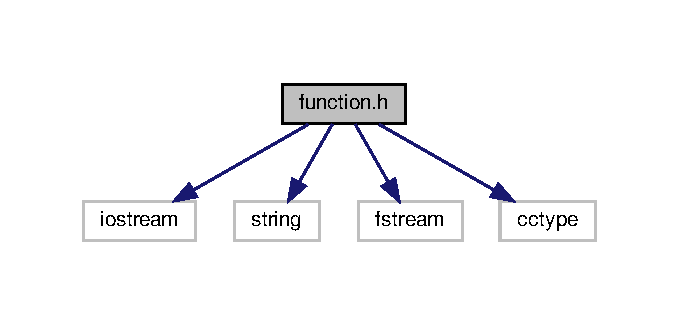
\includegraphics[width=326pt]{function_8h__incl}
\end{center}
\end{figure}
This graph shows which files directly or indirectly include this file\+:
\nopagebreak
\begin{figure}[H]
\begin{center}
\leavevmode
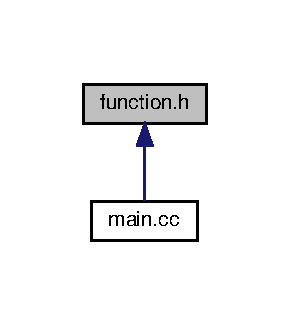
\includegraphics[width=139pt]{function_8h__dep__incl}
\end{center}
\end{figure}
\subsection*{Functions}
\begin{DoxyCompactItemize}
\item 
int \hyperlink{function_8h_acd3ebb697f805bec71bd06e6373bc4d1}{count\+Line} (string p\+Name)
\begin{DoxyCompactList}\small\item\em counts the total number of line in a string \end{DoxyCompactList}\item 
int \hyperlink{function_8h_a24555cd3b586589c2bfe4b97a1362a41}{count\+Char} (string p\+Name)
\begin{DoxyCompactList}\small\item\em counts the total number of char in a string, this function will count any except for white spaces \end{DoxyCompactList}\end{DoxyCompactItemize}


\subsection{Detailed Description}
library containing count\+Lines and count\+Char 

\begin{DoxyAuthor}{Author}
Gabriele Chiossi 
\end{DoxyAuthor}
\begin{DoxyDate}{Date}
December 3rd 2020 
\end{DoxyDate}


\subsection{Function Documentation}
\mbox{\Hypertarget{function_8h_a24555cd3b586589c2bfe4b97a1362a41}\label{function_8h_a24555cd3b586589c2bfe4b97a1362a41}} 
\index{function.\+h@{function.\+h}!count\+Char@{count\+Char}}
\index{count\+Char@{count\+Char}!function.\+h@{function.\+h}}
\subsubsection{\texorpdfstring{count\+Char()}{countChar()}}
{\footnotesize\ttfamily int count\+Char (\begin{DoxyParamCaption}\item[{string}]{p\+Name }\end{DoxyParamCaption})}



counts the total number of char in a string, this function will count any except for white spaces 


\begin{DoxyParams}{Parameters}
{\em p\+Name} & -\/ string passed to the function\\
\hline
\end{DoxyParams}
\begin{DoxyReturn}{Returns}
count, number of char total 
\end{DoxyReturn}
\mbox{\Hypertarget{function_8h_acd3ebb697f805bec71bd06e6373bc4d1}\label{function_8h_acd3ebb697f805bec71bd06e6373bc4d1}} 
\index{function.\+h@{function.\+h}!count\+Line@{count\+Line}}
\index{count\+Line@{count\+Line}!function.\+h@{function.\+h}}
\subsubsection{\texorpdfstring{count\+Line()}{countLine()}}
{\footnotesize\ttfamily int count\+Line (\begin{DoxyParamCaption}\item[{string}]{p\+Name }\end{DoxyParamCaption})}



counts the total number of line in a string 


\begin{DoxyParams}{Parameters}
{\em p\+Name} & -\/ string passed to the function\\
\hline
\end{DoxyParams}
\begin{DoxyReturn}{Returns}
count, number of lines total 
\end{DoxyReturn}

\hypertarget{main_8cc}{}\section{main.\+cc File Reference}
\label{main_8cc}\index{main.\+cc@{main.\+cc}}


main file  


{\ttfamily \#include $<$iostream$>$}\newline
{\ttfamily \#include $<$string$>$}\newline
{\ttfamily \#include $<$fstream$>$}\newline
{\ttfamily \#include $<$cctype$>$}\newline
{\ttfamily \#include \char`\"{}function.\+h\char`\"{}}\newline
Include dependency graph for main.\+cc\+:
\nopagebreak
\begin{figure}[H]
\begin{center}
\leavevmode
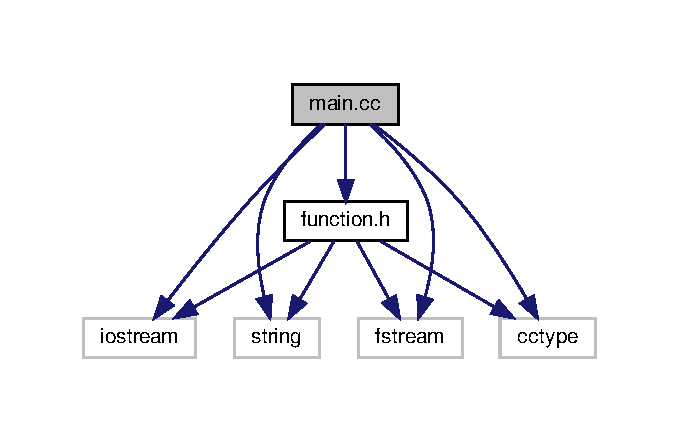
\includegraphics[width=326pt]{main_8cc__incl}
\end{center}
\end{figure}
\subsection*{Functions}
\begin{DoxyCompactItemize}
\item 
int \hyperlink{main_8cc_a3c04138a5bfe5d72780bb7e82a18e627}{main} (int argc, char $\ast$$\ast$argv)
\begin{DoxyCompactList}\small\item\em main function \end{DoxyCompactList}\end{DoxyCompactItemize}


\subsection{Detailed Description}
main file 

\begin{DoxyAuthor}{Author}
Gabriele Chiossi 
\end{DoxyAuthor}
\begin{DoxyDate}{Date}
December 3rd 2020 
\end{DoxyDate}


\subsection{Function Documentation}
\mbox{\Hypertarget{main_8cc_a3c04138a5bfe5d72780bb7e82a18e627}\label{main_8cc_a3c04138a5bfe5d72780bb7e82a18e627}} 
\index{main.\+cc@{main.\+cc}!main@{main}}
\index{main@{main}!main.\+cc@{main.\+cc}}
\subsubsection{\texorpdfstring{main()}{main()}}
{\footnotesize\ttfamily int main (\begin{DoxyParamCaption}\item[{int}]{argc,  }\item[{char $\ast$$\ast$}]{argv }\end{DoxyParamCaption})}



main function 


\begin{DoxyParams}{Parameters}
{\em int} & argc, and char $\ast$$\ast$argv\\
\hline
\end{DoxyParams}
\begin{DoxyReturn}{Returns}
integer 0 
\end{DoxyReturn}

%--- End generated contents ---

% Index
\backmatter
\newpage
\phantomsection
\clearemptydoublepage
\addcontentsline{toc}{chapter}{Index}
\printindex

\end{document}
